%\setlength{\parindent}{0pt}
\documentclass{article}
\usepackage{amsmath}
\usepackage{amssymb}
\usepackage{amsthm}
\usepackage{latexsym}

\usepackage{amsopn}
\DeclareMathOperator{\stab}{Stab}
\DeclareMathOperator{\perm}{Perm}
\DeclareMathOperator{\im}{im}
\DeclareMathOperator{\Aut}{Aut}
\DeclareMathOperator{\Hom}{Hom}
\DeclareMathOperator{\Perm}{Perm}
\DeclareMathOperator{\Frac}{Frac}
\DeclareMathOperator{\Pic}{Pic}
\DeclareMathOperator{\id}{id}
\DeclareMathOperator{\Tr}{Tr}
\DeclareMathOperator{\Spec}{Spec}
\DeclareMathOperator{\Proj}{Proj}
\DeclareMathOperator{\codim}{codim}


\usepackage[dvipsnames]{xcolor}
 
\definecolor{mypink1}{rgb}{0.858, 0.188, 0.478}

%\usepackage{color}
%\definecolor{keywordcolor}{rgb}{0.7, 0.1, 0.1}   % red
%\definecolor{commentcolor}{rgb}{0.4, 0.4, 0.4}   % grey
%\definecolor{symbolcolor}{rgb}{0.0, 0.1, 0.6}    % blue
%\definecolor{sortcolor}{rgb}{0.1, 0.5, 0.1}      % green
%\usepackage{listings}
%\def\lstlanguagefiles{lstlean.tex} 
%\lstset{language=lean}

\usepackage{enumitem}
\usepackage{tikz-cd}

\usepackage{tikz,tkz-euclide}
\usetikzlibrary{arrows,calc,intersections}
%\usetkzobj{all}

\usepackage{enumitem}
\usepackage[margin=2.2cm]{geometry}

\newcommand{\ideal}{\ensuremath{\triangleleft}}
\newcommand{\ol}{\ensuremath{\overline}}
\newcommand{\p}{\ensuremath{\mathfrak{p}}}
\newcommand{\m}{\ensuremath{\mathfrak{m}}}
\newcommand{\A}{\ensuremath{\mathbb{A}}}
\newcommand{\Z}{\ensuremath{\mathbb{Z}}}
\newcommand{\C}{\ensuremath{\mathbb{C}}}
\newcommand{\R}{\ensuremath{\mathbb{R}}}
\newcommand{\Q}{\ensuremath{\mathbb{Q}}}
\newcommand{\N}{\ensuremath{\mathbb{N}}}
\newcommand{\F}{\ensuremath{\mathbb{F}}}
\renewcommand{\P}{\ensuremath{\mathbb{P}}}
\newcommand{\Ox}{\mathscr{O}}

\newcommand{\q}{\ensuremath{\mathfrak{q}}}
%\newcommand{\N}{\ensuremath{\mathbb{N}}}

\usepackage{mathrsfs}
%\usepackage{fontspec}
%\usepackage{mathtools}
%\usepackage{unicode-math}

\usepackage{natbib}
\bibliographystyle{humannat}
%\bibliographystyle{unsrtnat}
%\bibliographystyle{abbrvnat}

\theoremstyle{definition}
\newcounter{dummy} \numberwithin{dummy}{section}
\newtheorem{lemma}[dummy]{Lemma}
%\newtheorem*{lemma*}[dummy]{Lemma}
\newtheorem{prop}[dummy]{Proposition}
\newtheorem{defi}[dummy]{Definition}
\newtheorem{cor}[dummy]{Corollary}
\newtheorem{example}[dummy]{Example}
\newtheorem{thm}[dummy]{Theorem}



\newcommand*{\DashedArrow}[1][]{\mathbin{\tikz [baseline=-0.25ex,-latex, dashed,#1] \draw [#1] (0pt,0.5ex) -- (1.3em,0.5ex);}}%
\newcommand{\dto}{\DashedArrow[->,densely dashed]}
%\newcommand{\da}{\DashedArrow}

%\usepackage{microtype}
\usepackage[activate={true,nocompatibility},final,tracking=true,kerning=true,spacing=true,factor=1100,stretch=10,shrink=10]{microtype}
\author{Louis Carlin -- u6384109}
\title{World Models with MDRNNs}
\usepackage[pdftex]{hyperref}
\hypersetup{
  colorlinks=true
}
\begin{document}
\maketitle
\begin{abstract}
In World Models (CITEME) David Ha et al describe an architecture allowing a computer agent to learn an internal model of its own environment.
Their model was powerful enough that agents could be trained in its dreamed simulation to achieve good performance in the original environment.
In this project I set out to create my own implimentation of the World Models architecture.

\end{abstract}

\section{Introduction}
%background stuff of other world models
When humans make decisions we often use an internal model of the problem at hand to inform our decision, allowing us to predict or calculate how the world might unfold based on our actions.
This model based approach may be something we are conscious of, as in the case of a chess player who uses their knowledge to look ahead and evaluate potential moves.
It also happens unconsciously, for example with batters in baseball who use an internal model to infer the position of the ball based on the the way the pitcher throws it, rather than reacting to the position of the ball milliseconds before it hits their bat.
In either case this internal model greatly improves our performance at these tasks.

In reinforcement learning we seek to develop computer agents which are capable of \textit{learning} to complete tasks.
Inspired by the success of own model based thought process we naturally seek to equip these agents with models of their environment.
There are several different ways this has been done.
Most traditionally an agent may be supplied with a model which has been handcrafted by a human. %TODO example
Unfortunately models made in this way are usually domain specific and thus the approach requires significant human involvement any time we try adapt an agent to learn in a new environment.
In a complex or partially unobservable environment it may even be infeasible for a human to equip an agent with a model adequately describing its world. %example?
More recently, deep reinforcement learning has circumvented this problem by increasing the complexity of the learned agent.
Agents constructed using architectures such as recurrent neural networks (RNNs) learn to perform complex computations.
In many cases they are able to harness this power to essentially learn their own model of the environment, allowing them to succeed at complex tasks without human intervention.
Deep reinforcement learning is not a complete solution however: training of complex agents is notoriously difficult, with what is known as the \textit{Credit Assignment Problem} often preventing agents from learning in environments with sparse reward signals.
A third approach, championed by Schmidthuber is to decouple the learning process, first learning a model $M$ and then using this model to train a controller $C$. %CITEME
The advantage of this approach is that complex models can be learned without worrying about credit assignment, allowing us to more easily train a comparatively simple controller.

World Models is a particularly simple implimentation of Schmidthuber's approach which has been shown to be remarkable effective at learning in image based environments. %CITEME
It breaks an agent into three components, the first two are vision $V$ and model $M$, and together these allow an agent to interpret and model its world.
The controller $C$ is then trained using both features of the environment and some of the internal knowledge of $M$.
Significantly, the internal model comprised of $V$ and $M$ is powerful enough to recreate a simulated version of the original environment, known as a \textit{dream}.
These dreams were close enough to the original environment that agents could be trained entirely inside a dream to perform well in the original environment.
In this project I primarily set out to investigate this part of World Models, which consists of the $V$ and $M$ components.

The structure of this report is as follows.
We begin with a brief overview of the World Models' architecture which serves as the primary motivation throughout this report.
In the subsequent three sections we discuss some of the theory behind each of the three components of World Models.
Finally, in the last section I discuss my own implementation and results.

\section{The World Models' Architecture}
%\subsection{Problem Description}
World Models uses a fairly standard description of the reinforcement learning problem.
Environments are broken down into discrete time steps.
At a time $t$ an agent receives a partial observation of the environment $o_t$ and are reward $r_t$.
The agent must then choose an action $a_t$ from a set of possible actions.
In an \textit{episodic} task where there are only ever finitely many time steps the agent's task is to pick $a_t$ such that the sum of future rewards is maximised.
In a \textit{continuing} task where the environment is ongoing an agent instead picks $a_t$ to maximise a weighted sum of future rewards where more distant rewards are weighted with decreasing values to ensure the sum converges.

Although Schmidthuber's original ideas apply much more generally the World Models architecture is adapted to image based problems where the observation $o_t$ is a two dimensional image.
Environments such as these are navigated with ease by humans playing videogames, yet still remain a challenge in reinforcement learning.
David Ha et al. empirically tested their model in two different environments.
The first one was \texttt{CarRacing-v0} where an agent must learn to drive a car based on a top-down image of the racing track. %CITEME
Here the agent is rewarded more the more tiles they visit, which incentivises speedier and more accurate driving.
The second environment was \texttt{VizDoom: Take Cover} where an agent learns to dodge fireballs thrown at it by demons in the 3D environment of the videogame Doom.
In this environment observations are first person images from the perspective of the agent and rewards are simply given to the agent based on survival time.
%TODO picture of both environments

\begin{figure}[h]
  \centering
  \begin{minipage}{0.45\textwidth}
      \centering
      \includegraphics[width=0.9\textwidth]{CarRacing-v0.jpeg} % first figure itself
      \caption{An observation from the \texttt{CarRacing-v0} environment}
  \end{minipage}\hfill
  \begin{minipage}{0.45\textwidth}
      \centering
      \includegraphics[width=0.9\textwidth]{VizDoom.jpeg} % second figure itself
      \caption{An observation from the \texttt{VizDoom: Take Cover} environment}
  \end{minipage}
\end{figure}

%overview of model V-M-C
The World Models' architecture is split into three components: \textit{Vision (V), Memory (M)}, and \textit{Controller (C)}.
The Vision component is comprised of an variational autoencoder.
It takes in an image observation $o$ and gives a much smaller vector $z$, known as the \textit{latent representation}, which we can think of as a compressed version of $o$.
The idea behind this compression is that it will be easier to learn an internal model of the dynamics of this smaller latent state than to try predict the evolution of the observation images. 
The Memory component is a Mixture Density Reccurrent Neural Net (MDRNN) and forms the bulk of agent's internal model.
Given the current latent state $z_t$, an action $a_t$, and its own memory output $h_{t}$ from the previous state, $M$ is trained to predict the distribution of the next latent state $z_{t+1}$ will be given that action.
That is, $M$ learns the distribution $p(z_{t+1} | z_t, a_t, h_t)$.
Finally, the Controller learns a simple linear mapping from the latent state $z$ and previous memory state $h$ to an action. 

\begin{figure}[h]
  \centering


\tikzset{every picture/.style={line width=0.75pt}} %set default line width to 0.75pt        

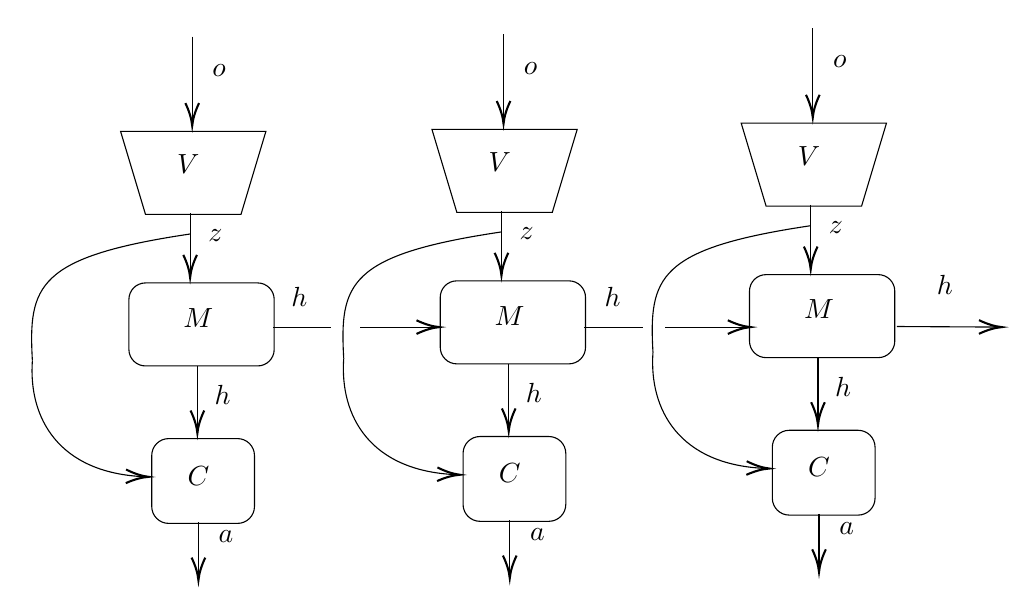
\begin{tikzpicture}[x=0.75pt,y=0.75pt,yscale=-1,xscale=1]
%uncomment if require: \path (0,300); %set diagram left start at 0, and has height of 300

%Shape: Trapezoid [id:dp8835259262509831] 
\draw   (214,73) -- (202,113) -- (156,113) -- (144,73) -- cycle ;
%Rounded Rect [id:dp0285219553359235] 
\draw   (148,154) .. controls (148,149.58) and (151.58,146) .. (156,146) -- (210,146) .. controls (214.42,146) and (218,149.58) .. (218,154) -- (218,178) .. controls (218,182.42) and (214.42,186) .. (210,186) -- (156,186) .. controls (151.58,186) and (148,182.42) .. (148,178) -- cycle ;
%Rounded Rect [id:dp3457403063059383] 
\draw   (159,229.17) .. controls (159,224.66) and (162.66,221) .. (167.17,221) -- (200.33,221) .. controls (204.84,221) and (208.5,224.66) .. (208.5,229.17) -- (208.5,253.69) .. controls (208.5,258.2) and (204.84,261.86) .. (200.33,261.86) -- (167.17,261.86) .. controls (162.66,261.86) and (159,258.2) .. (159,253.69) -- cycle ;
%Straight Lines [id:da5830231307220126] 
\draw    (181,186) -- (181,216.43) ;
\draw [shift={(181,218.43)}, rotate = 270] [color={rgb, 255:red, 0; green, 0; blue, 0 }  ][line width=0.75]    (10.93,-3.29) .. controls (6.95,-1.4) and (3.31,-0.3) .. (0,0) .. controls (3.31,0.3) and (6.95,1.4) .. (10.93,3.29)   ;
%Straight Lines [id:da21875827228445366] 
\draw    (177.5,112.43) -- (177.5,141.43) ;
\draw [shift={(177.5,143.43)}, rotate = 270] [color={rgb, 255:red, 0; green, 0; blue, 0 }  ][line width=0.75]    (10.93,-3.29) .. controls (6.95,-1.4) and (3.31,-0.3) .. (0,0) .. controls (3.31,0.3) and (6.95,1.4) .. (10.93,3.29)   ;
%Curve Lines [id:da18494477060365933] 
\draw    (177.5,122.43) .. controls (103.5,133.43) and (99.5,147.43) .. (101.5,183.43) ;
%Curve Lines [id:da3167428765764193] 
\draw    (101.5,183.43) .. controls (99.53,211.01) and (114.05,237.62) .. (155.58,239.37) ;
\draw [shift={(157.5,239.43)}, rotate = 181.33] [color={rgb, 255:red, 0; green, 0; blue, 0 }  ][line width=0.75]    (10.93,-3.29) .. controls (6.95,-1.4) and (3.31,-0.3) .. (0,0) .. controls (3.31,0.3) and (6.95,1.4) .. (10.93,3.29)   ;
%Straight Lines [id:da13659803234644108] 
\draw    (178.5,27.29) -- (178.5,68.29) ;
\draw [shift={(178.5,70.29)}, rotate = 270] [color={rgb, 255:red, 0; green, 0; blue, 0 }  ][line width=0.75]    (10.93,-3.29) .. controls (6.95,-1.4) and (3.31,-0.3) .. (0,0) .. controls (3.31,0.3) and (6.95,1.4) .. (10.93,3.29)   ;
%Straight Lines [id:da7386372433419905] 
\draw    (181.5,261.29) -- (181.5,287.29) ;
\draw [shift={(181.5,289.29)}, rotate = 270] [color={rgb, 255:red, 0; green, 0; blue, 0 }  ][line width=0.75]    (10.93,-3.29) .. controls (6.95,-1.4) and (3.31,-0.3) .. (0,0) .. controls (3.31,0.3) and (6.95,1.4) .. (10.93,3.29)   ;
%Shape: Trapezoid [id:dp1462361877942473] 
\draw   (364,72) -- (352,112) -- (306,112) -- (294,72) -- cycle ;
%Rounded Rect [id:dp18606077574272506] 
\draw   (298,153) .. controls (298,148.58) and (301.58,145) .. (306,145) -- (360,145) .. controls (364.42,145) and (368,148.58) .. (368,153) -- (368,177) .. controls (368,181.42) and (364.42,185) .. (360,185) -- (306,185) .. controls (301.58,185) and (298,181.42) .. (298,177) -- cycle ;
%Rounded Rect [id:dp4652776111951933] 
\draw   (309,228.17) .. controls (309,223.66) and (312.66,220) .. (317.17,220) -- (350.33,220) .. controls (354.84,220) and (358.5,223.66) .. (358.5,228.17) -- (358.5,252.69) .. controls (358.5,257.2) and (354.84,260.86) .. (350.33,260.86) -- (317.17,260.86) .. controls (312.66,260.86) and (309,257.2) .. (309,252.69) -- cycle ;
%Straight Lines [id:da9151430963452045] 
\draw    (331,185) -- (331,215.43) ;
\draw [shift={(331,217.43)}, rotate = 270] [color={rgb, 255:red, 0; green, 0; blue, 0 }  ][line width=0.75]    (10.93,-3.29) .. controls (6.95,-1.4) and (3.31,-0.3) .. (0,0) .. controls (3.31,0.3) and (6.95,1.4) .. (10.93,3.29)   ;
%Straight Lines [id:da07699090937850928] 
\draw    (327.5,111.43) -- (327.5,140.43) ;
\draw [shift={(327.5,142.43)}, rotate = 270] [color={rgb, 255:red, 0; green, 0; blue, 0 }  ][line width=0.75]    (10.93,-3.29) .. controls (6.95,-1.4) and (3.31,-0.3) .. (0,0) .. controls (3.31,0.3) and (6.95,1.4) .. (10.93,3.29)   ;
%Curve Lines [id:da8115724577514165] 
\draw    (327.5,121.43) .. controls (253.5,132.43) and (249.5,146.43) .. (251.5,182.43) ;
%Curve Lines [id:da6705210586592285] 
\draw    (251.5,182.43) .. controls (249.53,210.01) and (264.05,236.62) .. (305.58,238.37) ;
\draw [shift={(307.5,238.43)}, rotate = 181.33] [color={rgb, 255:red, 0; green, 0; blue, 0 }  ][line width=0.75]    (10.93,-3.29) .. controls (6.95,-1.4) and (3.31,-0.3) .. (0,0) .. controls (3.31,0.3) and (6.95,1.4) .. (10.93,3.29)   ;
%Straight Lines [id:da2713335277085913] 
\draw    (328.5,26.29) -- (328.5,67.29) ;
\draw [shift={(328.5,69.29)}, rotate = 270] [color={rgb, 255:red, 0; green, 0; blue, 0 }  ][line width=0.75]    (10.93,-3.29) .. controls (6.95,-1.4) and (3.31,-0.3) .. (0,0) .. controls (3.31,0.3) and (6.95,1.4) .. (10.93,3.29)   ;
%Straight Lines [id:da018255342957326226] 
\draw    (331.5,260.29) -- (331.5,286.29) ;
\draw [shift={(331.5,288.29)}, rotate = 270] [color={rgb, 255:red, 0; green, 0; blue, 0 }  ][line width=0.75]    (10.93,-3.29) .. controls (6.95,-1.4) and (3.31,-0.3) .. (0,0) .. controls (3.31,0.3) and (6.95,1.4) .. (10.93,3.29)   ;
%Shape: Trapezoid [id:dp2430591295177642] 
\draw   (513,69) -- (501,109) -- (455,109) -- (443,69) -- cycle ;
%Rounded Rect [id:dp39814637506948647] 
\draw   (447,150) .. controls (447,145.58) and (450.58,142) .. (455,142) -- (509,142) .. controls (513.42,142) and (517,145.58) .. (517,150) -- (517,174) .. controls (517,178.42) and (513.42,182) .. (509,182) -- (455,182) .. controls (450.58,182) and (447,178.42) .. (447,174) -- cycle ;
%Rounded Rect [id:dp21706991468861547] 
\draw   (458,225.17) .. controls (458,220.66) and (461.66,217) .. (466.17,217) -- (499.33,217) .. controls (503.84,217) and (507.5,220.66) .. (507.5,225.17) -- (507.5,249.69) .. controls (507.5,254.2) and (503.84,257.86) .. (499.33,257.86) -- (466.17,257.86) .. controls (461.66,257.86) and (458,254.2) .. (458,249.69) -- cycle ;
%Straight Lines [id:da2885218987388809] 
\draw    (480,182) -- (480,212.43) ;
\draw [shift={(480,214.43)}, rotate = 270] [color={rgb, 255:red, 0; green, 0; blue, 0 }  ][line width=0.75]    (10.93,-3.29) .. controls (6.95,-1.4) and (3.31,-0.3) .. (0,0) .. controls (3.31,0.3) and (6.95,1.4) .. (10.93,3.29)   ;
%Straight Lines [id:da415487537189946] 
\draw    (476.5,108.43) -- (476.5,137.43) ;
\draw [shift={(476.5,139.43)}, rotate = 270] [color={rgb, 255:red, 0; green, 0; blue, 0 }  ][line width=0.75]    (10.93,-3.29) .. controls (6.95,-1.4) and (3.31,-0.3) .. (0,0) .. controls (3.31,0.3) and (6.95,1.4) .. (10.93,3.29)   ;
%Curve Lines [id:da9113104095636424] 
\draw    (476.5,118.43) .. controls (402.5,129.43) and (398.5,143.43) .. (400.5,179.43) ;
%Curve Lines [id:da9743514631293164] 
\draw    (400.5,179.43) .. controls (398.53,207.01) and (413.05,233.62) .. (454.58,235.37) ;
\draw [shift={(456.5,235.43)}, rotate = 181.33] [color={rgb, 255:red, 0; green, 0; blue, 0 }  ][line width=0.75]    (10.93,-3.29) .. controls (6.95,-1.4) and (3.31,-0.3) .. (0,0) .. controls (3.31,0.3) and (6.95,1.4) .. (10.93,3.29)   ;
%Straight Lines [id:da7539268513899835] 
\draw    (477.5,23.29) -- (477.5,64.29) ;
\draw [shift={(477.5,66.29)}, rotate = 270] [color={rgb, 255:red, 0; green, 0; blue, 0 }  ][line width=0.75]    (10.93,-3.29) .. controls (6.95,-1.4) and (3.31,-0.3) .. (0,0) .. controls (3.31,0.3) and (6.95,1.4) .. (10.93,3.29)   ;
%Straight Lines [id:da06251428437526796] 
\draw    (480.5,257.29) -- (480.5,283.29) ;
\draw [shift={(480.5,285.29)}, rotate = 270] [color={rgb, 255:red, 0; green, 0; blue, 0 }  ][line width=0.75]    (10.93,-3.29) .. controls (6.95,-1.4) and (3.31,-0.3) .. (0,0) .. controls (3.31,0.3) and (6.95,1.4) .. (10.93,3.29)   ;
%Straight Lines [id:da4924611031680366] 
\draw    (217.5,167.29) -- (245.5,167.29) ;
%Straight Lines [id:da3927822338264424] 
\draw    (259.5,167.29) -- (295.5,167.29) ;
\draw [shift={(297.5,167.29)}, rotate = 180] [color={rgb, 255:red, 0; green, 0; blue, 0 }  ][line width=0.75]    (10.93,-3.29) .. controls (6.95,-1.4) and (3.31,-0.3) .. (0,0) .. controls (3.31,0.3) and (6.95,1.4) .. (10.93,3.29)   ;
%Straight Lines [id:da4299695706705984] 
\draw    (367.5,167.29) -- (395.5,167.29) ;
%Straight Lines [id:da7674556510413473] 
\draw    (406.5,167.29) -- (445.5,167.29) ;
\draw [shift={(447.5,167.29)}, rotate = 180] [color={rgb, 255:red, 0; green, 0; blue, 0 }  ][line width=0.75]    (10.93,-3.29) .. controls (6.95,-1.4) and (3.31,-0.3) .. (0,0) .. controls (3.31,0.3) and (6.95,1.4) .. (10.93,3.29)   ;
%Straight Lines [id:da9354612324356146] 
\draw    (518,167) -- (566.5,167.27) ;
\draw [shift={(568.5,167.29)}, rotate = 180.32] [color={rgb, 255:red, 0; green, 0; blue, 0 }  ][line width=0.75]    (10.93,-3.29) .. controls (6.95,-1.4) and (3.31,-0.3) .. (0,0) .. controls (3.31,0.3) and (6.95,1.4) .. (10.93,3.29)   ;

% Text Node
\draw (187,39.4) node [anchor=north west][inner sep=0.75pt]    {$o$};
% Text Node
\draw (185,119) node [anchor=north west][inner sep=0.75pt]   [align=left] {$\displaystyle z$};
% Text Node
\draw (170,83) node [anchor=north west][inner sep=0.75pt]   [align=left] {$\displaystyle V$};
% Text Node
\draw (173,157) node [anchor=north west][inner sep=0.75pt]   [align=left] {$\displaystyle M$};
% Text Node
\draw (175,233) node [anchor=north west][inner sep=0.75pt]   [align=left] {$\displaystyle C$};
% Text Node
\draw (190,264) node [anchor=north west][inner sep=0.75pt]   [align=left] {$\displaystyle a$};
% Text Node
\draw (188,194) node [anchor=north west][inner sep=0.75pt]   [align=left] {$\displaystyle h$};
% Text Node
\draw (337,38.4) node [anchor=north west][inner sep=0.75pt]    {$o$};
% Text Node
\draw (335,118) node [anchor=north west][inner sep=0.75pt]   [align=left] {$\displaystyle z$};
% Text Node
\draw (320,82) node [anchor=north west][inner sep=0.75pt]   [align=left] {$\displaystyle V$};
% Text Node
\draw (323,156) node [anchor=north west][inner sep=0.75pt]   [align=left] {$\displaystyle M$};
% Text Node
\draw (325,232) node [anchor=north west][inner sep=0.75pt]   [align=left] {$\displaystyle C$};
% Text Node
\draw (340,263) node [anchor=north west][inner sep=0.75pt]   [align=left] {$\displaystyle a$};
% Text Node
\draw (338,193) node [anchor=north west][inner sep=0.75pt]   [align=left] {$\displaystyle h$};
% Text Node
\draw (486,35.4) node [anchor=north west][inner sep=0.75pt]    {$o$};
% Text Node
\draw (484,115) node [anchor=north west][inner sep=0.75pt]   [align=left] {$\displaystyle z$};
% Text Node
\draw (469,79) node [anchor=north west][inner sep=0.75pt]   [align=left] {$\displaystyle V$};
% Text Node
\draw (472,153) node [anchor=north west][inner sep=0.75pt]   [align=left] {$\displaystyle M$};
% Text Node
\draw (474,229) node [anchor=north west][inner sep=0.75pt]   [align=left] {$\displaystyle C$};
% Text Node
\draw (489,260) node [anchor=north west][inner sep=0.75pt]   [align=left] {$\displaystyle a$};
% Text Node
\draw (487,190) node [anchor=north west][inner sep=0.75pt]   [align=left] {$\displaystyle h$};
% Text Node
\draw (225,147) node [anchor=north west][inner sep=0.75pt]   [align=left] {$\displaystyle h$};
% Text Node
\draw (376,147) node [anchor=north west][inner sep=0.75pt]   [align=left] {$\displaystyle h$};
% Text Node
\draw (536,141) node [anchor=north west][inner sep=0.75pt]   [align=left] {$\displaystyle h$};


\end{tikzpicture}
      \caption{The three components of World Models: Vision, Memory, and Controller}
\end{figure}

%deep reinforcment learning learns models but struggles with credit assignment



\section{Vision}
%autoencoders (show old example?)
%show new example
The Vision component consists of a Variational Autoencoder (VAE) which simultaneously trains both an encoder and decoder.
The encoder learns to compress image observations into smaller latent representations and the decoder learns to reconstruct the original observations from the latent representations.
VAEs are not particularly new technology, however their use in World Models is perhaps the most novel component of the paper. %TODO mention previous attempts, lack of stability
Observations in the two environments investigated by Ha et al are $64 \times 64$ pixel images with 3 colour channels, and thus represented by 12288 dimensional vectors.
The Vision component manages to compress each observation into 32 dimensional latent representation, which can then be used...



\subsection{Autoencoders}
Autoencoders allow us to learn more efficient representations of data.
One way to think of them\footnote{Autoencoders actually have a variety of other applications such as image infilling, image segmentation, and denoising, but we will not discuss these here.} is as learning a lossy compression algorithm which is heuristically tailored torwards the data it has been trained on.
Autoencoders consist of two separate models: an encoder and a decoder. %CITEME image infilling, image segmentation, and denoising
The encoder is a neural net which takes in a high dimensional input $x$, such as an image, and returns a lower dimensional vector $z$ which is supposed to summarise the information contained in $x$.
The decoder takes this smaller vector $z$ as input and returns $\widetilde{x}$, an approximate reconstruction of $x$.
The combined Encoder-Decoder network is trained simultaneously by gradient descent with backpropagation.
The loss function used is known as a \textit{reconstruction loss} and is typically a measure of similarity between $x$ and $\widetilde{x}$, such as least squares.
Since the prediction compared to in the loss function is just the original input $x$ autoencoders are able to learn efficient representations in a completely unsupervised manner.


\begin{figure}[h]
  \centering


\tikzset{every picture/.style={line width=0.75pt}} %set default line width to 0.75pt        

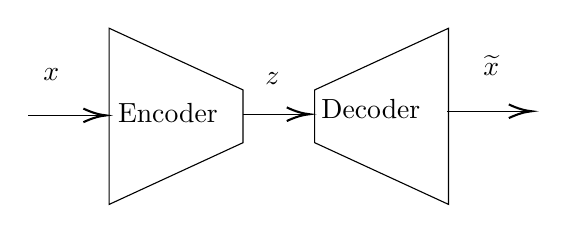
\begin{tikzpicture}[x=0.75pt,y=0.75pt,yscale=-1,xscale=1]
%uncomment if require: \path (0,300); %set diagram left start at 0, and has height of 300

%Shape: Trapezoid [id:dp8541203132727615] 
\draw   (151,77) -- (215.5,106.73) -- (215.5,132.14) -- (151,161.88) -- cycle ;
%Shape: Trapezoid [id:dp018706469204115228] 
\draw   (314.5,161.88) -- (250,132.14) -- (250,106.73) -- (314.5,77) -- cycle ;
%Straight Lines [id:da8293223382895447] 
\draw    (215.5,118.43) -- (245.5,118.43) ;
\draw [shift={(247.5,118.43)}, rotate = 180] [color={rgb, 255:red, 0; green, 0; blue, 0 }  ][line width=0.75]    (10.93,-3.29) .. controls (6.95,-1.4) and (3.31,-0.3) .. (0,0) .. controls (3.31,0.3) and (6.95,1.4) .. (10.93,3.29)   ;
%Straight Lines [id:da18164573910193638] 
\draw    (112,119) -- (147.5,119) ;
\draw [shift={(149.5,119)}, rotate = 180] [color={rgb, 255:red, 0; green, 0; blue, 0 }  ][line width=0.75]    (10.93,-3.29) .. controls (6.95,-1.4) and (3.31,-0.3) .. (0,0) .. controls (3.31,0.3) and (6.95,1.4) .. (10.93,3.29)   ;
%Straight Lines [id:da12573110589897274] 
\draw    (314,117) -- (352.5,117) ;
\draw [shift={(354.5,117)}, rotate = 180] [color={rgb, 255:red, 0; green, 0; blue, 0 }  ][line width=0.75]    (10.93,-3.29) .. controls (6.95,-1.4) and (3.31,-0.3) .. (0,0) .. controls (3.31,0.3) and (6.95,1.4) .. (10.93,3.29)   ;

% Text Node
\draw (154,112) node [anchor=north west][inner sep=0.75pt]   [align=left] {Encoder};
% Text Node
\draw (118,95) node [anchor=north west][inner sep=0.75pt]   [align=left] {$\displaystyle x$};
% Text Node
\draw (225,97) node [anchor=north west][inner sep=0.75pt]   [align=left] {$\displaystyle z$};
% Text Node
\draw (252,109.73) node [anchor=north west][inner sep=0.75pt]   [align=left] {Decoder};
% Text Node
\draw (330,89) node [anchor=north west][inner sep=0.75pt]   [align=left] {$\displaystyle \widetilde{x}$};


\end{tikzpicture}
\caption{An autoencoder}
\end{figure}

Network architecture for the Encoder and Decoder can vary wildly depending on the area of application.
In image processing it is standard practice to use 2D convolutional layers rather than fully connected dense layers.
These convolutional layers vastly reduce the number of weights needed, making training feasible in cases where a fully connected network would struggle.
They do this be reusing weights on the principle that we are interested in common features of images, such as edges and colour gradients, rather than features localised to specific pixels.
Convolutional layers consist of many filter channels.
Each filter channel is computed by dragging a matrix of numbers known as a \textit{kernel} across the image and taking its dot product with the image at the different points.
Strictly the kernels are actually 3 dimensional matrices to account for the fact that our images and hidden cells have multiple channels.

\begin{figure}[h]
  \centering
  \includegraphics[scale=0.4]{2conv.png}
  \caption{A $3 \times 3$ kernel (shaded) is convolved over a $5 \times 5$ image (lower) which has been padded with zeros to a $7 \times 7$ matrix. The resulting output is also a $5 \times 5$ matrix.}
\end{figure}%CITEME towardsdatascience

A question one might be tempted to ask is what happens if we apply take the Decoder and apply it to a $z$ which has been randomly generated rather than coming via the Encoder.
We might hope that the image reconstructed by the Decoder resembles images from our original dataset.
If this were the case then we would be able to generate new images with this technique.
Unfortunately there is nothing to really guarantee this works.
If we think of our dataset as following some distribution $p(x)$ then there is not much we can say about the distribution of latent variables $p(z)$, and thus we cannot hope to directly sample a $z$ from this distribution, meaning we cannot sample a $z$ which might give a realistic $\widetilde{x}$.
Variational autoencoders are essentially designed to tackle this exact problem.

%TODO image pokemon?

\subsection{Variational Autoencoders}

Variational autoencoders consist of a convolutional Encoder and Decoder and work on a similar principle to normal autoencoders.
The encoder again takes in a high dimensional input $x$ such as an image.
However, instead of outputting a vector encoding $z$ the Encoder learns to output a distribution $q(z|x)$ of encodings representing $x$.
We require that $q(z|x)$ is a normal distribution with diagonal covariance so that the encoder actually outputs a vector twice the dimension of $z$, whose components represent the mean and covariance of $q(z|x)$.
We then sample a $z$ from this distribution and give this to the Decoder which decodes as normal to produce a reconstruction $\widetilde{x}$.
This added element of randomness is useful for reasons we will discuss shortly.

\begin{figure}[h]
  \centering


  \tikzset{every picture/.style={line width=0.75pt}} %set default line width to 0.75pt        

  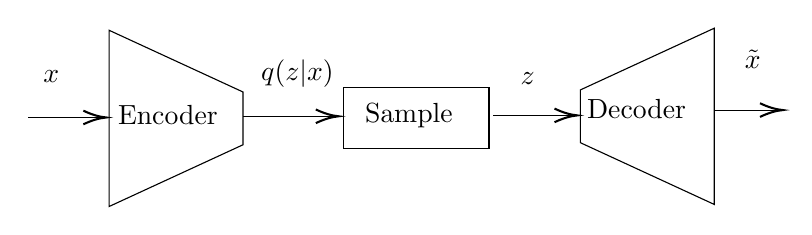
\begin{tikzpicture}[x=0.75pt,y=0.75pt,yscale=-1,xscale=1]
  %uncomment if require: \path (0,300); %set diagram left start at 0, and has height of 300
  
  %Shape: Trapezoid [id:dp8541203132727615] 
  \draw   (151,77) -- (215.5,106.73) -- (215.5,132.14) -- (151,161.88) -- cycle ;
  %Shape: Trapezoid [id:dp018706469204115228] 
  \draw   (442.5,160.88) -- (378,131.14) -- (378,105.73) -- (442.5,76) -- cycle ;
  %Straight Lines [id:da8293223382895447] 
  \draw    (215.5,118.43) -- (259.5,118.43) ;
  \draw [shift={(261.5,118.43)}, rotate = 180] [color={rgb, 255:red, 0; green, 0; blue, 0 }  ][line width=0.75]    (10.93,-3.29) .. controls (6.95,-1.4) and (3.31,-0.3) .. (0,0) .. controls (3.31,0.3) and (6.95,1.4) .. (10.93,3.29)   ;
  %Straight Lines [id:da18164573910193638] 
  \draw    (112,119) -- (147.5,119) ;
  \draw [shift={(149.5,119)}, rotate = 180] [color={rgb, 255:red, 0; green, 0; blue, 0 }  ][line width=0.75]    (10.93,-3.29) .. controls (6.95,-1.4) and (3.31,-0.3) .. (0,0) .. controls (3.31,0.3) and (6.95,1.4) .. (10.93,3.29)   ;
  %Straight Lines [id:da12573110589897274] 
  \draw    (336,118) -- (374.5,118) ;
  \draw [shift={(376.5,118)}, rotate = 180] [color={rgb, 255:red, 0; green, 0; blue, 0 }  ][line width=0.75]    (10.93,-3.29) .. controls (6.95,-1.4) and (3.31,-0.3) .. (0,0) .. controls (3.31,0.3) and (6.95,1.4) .. (10.93,3.29)   ;
  %Shape: Rectangle [id:dp9631400703948827] 
  \draw   (264,104.43) -- (334,104.43) -- (334,134) -- (264,134) -- cycle ;
  %Straight Lines [id:da9905140662945862] 
  \draw    (442.5,115.43) -- (473.5,115.43) ;
  \draw [shift={(475.5,115.43)}, rotate = 180] [color={rgb, 255:red, 0; green, 0; blue, 0 }  ][line width=0.75]    (10.93,-3.29) .. controls (6.95,-1.4) and (3.31,-0.3) .. (0,0) .. controls (3.31,0.3) and (6.95,1.4) .. (10.93,3.29)   ;
  
  % Text Node
  \draw (154,112) node [anchor=north west][inner sep=0.75pt]   [align=left] {Encoder};
  % Text Node
  \draw (118,95) node [anchor=north west][inner sep=0.75pt]   [align=left] {$\displaystyle x$};
  % Text Node
  \draw (223,90) node [anchor=north west][inner sep=0.75pt]   [align=left] {$\displaystyle q(z|x)$};
  % Text Node
  \draw (380,108.73) node [anchor=north west][inner sep=0.75pt]   [align=left] {Decoder};
  % Text Node
  \draw (456,85) node [anchor=north west][inner sep=0.75pt]   [align=left] {$\displaystyle \tilde{x}$};
  % Text Node
  \draw (273,111) node [anchor=north west][inner sep=0.75pt]   [align=left] {Sample};
  % Text Node
  \draw (348,96) node [anchor=north west][inner sep=0.75pt]   [align=left] {$\displaystyle z$};
  
  
  \end{tikzpicture}
  \caption{A variational autoencoder}
\end{figure}

We would like to train the variational autoencoder the same way we train traditional autoencoders, using backpropagation to compute the gradient of a loss function.
However, we cannot do this directly since there is no way to evaluate gradients through the random sampling process.
We get around this issue with something known as the ``reparamaterisation trick''.
Any time a datapoint is seen during training we sample an $\epsilon$ from the unit variance, zero mean gaussian with dimension the same as $z$.
Given output vectors $\mu$ and $\sigma$ from the Encoder representing the mean and covariance of $q(z|x)$ respectively, we find that $z = \mu + \sigma \odot \epsilon$ is distributed according to $q(z|x)$.
Then for each individual datapoint we treat its sampled $\epsilon$ as a constant so that $z$ is just a function of the original input and the Encoder's weights.
This allows us to give the resulting $z$ to the Decoder and compute the gradient of the resulting loss function via backpropagation.
%one of which is that it allows us control over the distribution of latent vector 

\begin{figure}[h]
  \centering








  \tikzset{every picture/.style={line width=0.75pt}} %set default line width to 0.75pt        

  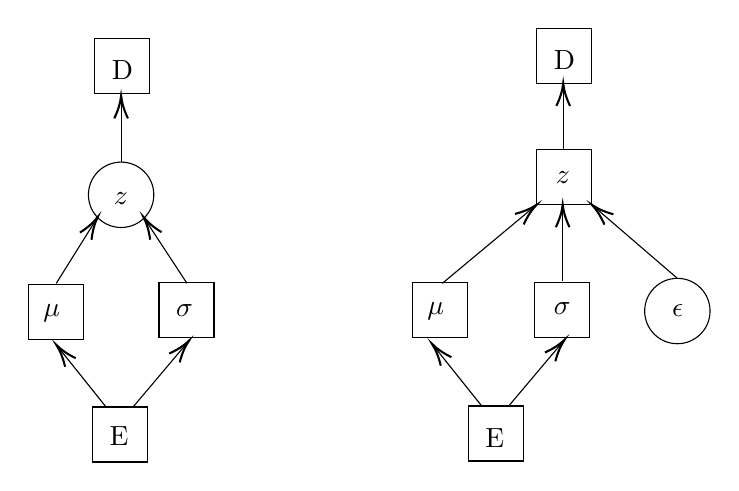
\begin{tikzpicture}[x=0.75pt,y=0.75pt,yscale=-1,xscale=1]
  %uncomment if require: \path (0,300); %set diagram left start at 0, and has height of 300
  
  %Shape: Square [id:dp31964573484955117] 
  \draw   (108,190) -- (134.5,190) -- (134.5,216.5) -- (108,216.5) -- cycle ;
  %Shape: Square [id:dp3315381522116503] 
  \draw   (171,189) -- (197.5,189) -- (197.5,215.5) -- (171,215.5) -- cycle ;
  %Shape: Circle [id:dp5157137150601787] 
  \draw   (137,146.75) .. controls (137,138.05) and (144.05,131) .. (152.75,131) .. controls (161.45,131) and (168.5,138.05) .. (168.5,146.75) .. controls (168.5,155.45) and (161.45,162.5) .. (152.75,162.5) .. controls (144.05,162.5) and (137,155.45) .. (137,146.75) -- cycle ;
  %Shape: Square [id:dp05107603102822389] 
  \draw   (293,189) -- (319.5,189) -- (319.5,215.5) -- (293,215.5) -- cycle ;
  %Shape: Square [id:dp22569528245966897] 
  \draw   (352,189) -- (378.5,189) -- (378.5,215.5) -- (352,215.5) -- cycle ;
  %Shape: Square [id:dp9307723856742833] 
  \draw   (353,125) -- (379.5,125) -- (379.5,151.5) -- (353,151.5) -- cycle ;
  %Shape: Circle [id:dp39963963544757175] 
  \draw   (405,202.75) .. controls (405,194.05) and (412.05,187) .. (420.75,187) .. controls (429.45,187) and (436.5,194.05) .. (436.5,202.75) .. controls (436.5,211.45) and (429.45,218.5) .. (420.75,218.5) .. controls (412.05,218.5) and (405,211.45) .. (405,202.75) -- cycle ;
  %Straight Lines [id:da5853904219054253] 
  \draw    (121.5,189.43) -- (140.44,159.12) ;
  \draw [shift={(141.5,157.43)}, rotate = 482.01] [color={rgb, 255:red, 0; green, 0; blue, 0 }  ][line width=0.75]    (10.93,-3.29) .. controls (6.95,-1.4) and (3.31,-0.3) .. (0,0) .. controls (3.31,0.3) and (6.95,1.4) .. (10.93,3.29)   ;
  %Straight Lines [id:da029718248550361537] 
  \draw    (184.5,189.43) -- (164.6,159.1) ;
  \draw [shift={(163.5,157.43)}, rotate = 416.73] [color={rgb, 255:red, 0; green, 0; blue, 0 }  ][line width=0.75]    (10.93,-3.29) .. controls (6.95,-1.4) and (3.31,-0.3) .. (0,0) .. controls (3.31,0.3) and (6.95,1.4) .. (10.93,3.29)   ;
  %Straight Lines [id:da21889214167912363] 
  \draw    (152.75,131) -- (152.75,101) ;
  \draw [shift={(152.75,99)}, rotate = 450] [color={rgb, 255:red, 0; green, 0; blue, 0 }  ][line width=0.75]    (10.93,-3.29) .. controls (6.95,-1.4) and (3.31,-0.3) .. (0,0) .. controls (3.31,0.3) and (6.95,1.4) .. (10.93,3.29)   ;
  %Straight Lines [id:da4460377874666688] 
  \draw    (307.5,189.43) -- (351.46,152.78) ;
  \draw [shift={(353,151.5)}, rotate = 500.19] [color={rgb, 255:red, 0; green, 0; blue, 0 }  ][line width=0.75]    (10.93,-3.29) .. controls (6.95,-1.4) and (3.31,-0.3) .. (0,0) .. controls (3.31,0.3) and (6.95,1.4) .. (10.93,3.29)   ;
  %Straight Lines [id:da6243739236469146] 
  \draw    (365.5,188.43) -- (365.5,153.43) ;
  \draw [shift={(365.5,151.43)}, rotate = 450] [color={rgb, 255:red, 0; green, 0; blue, 0 }  ][line width=0.75]    (10.93,-3.29) .. controls (6.95,-1.4) and (3.31,-0.3) .. (0,0) .. controls (3.31,0.3) and (6.95,1.4) .. (10.93,3.29)   ;
  %Straight Lines [id:da8887544337702149] 
  \draw    (420.75,187) -- (381.02,152.8) ;
  \draw [shift={(379.5,151.5)}, rotate = 400.72] [color={rgb, 255:red, 0; green, 0; blue, 0 }  ][line width=0.75]    (10.93,-3.29) .. controls (6.95,-1.4) and (3.31,-0.3) .. (0,0) .. controls (3.31,0.3) and (6.95,1.4) .. (10.93,3.29)   ;
  %Straight Lines [id:da6173989757165841] 
  \draw    (365.75,125) -- (365.75,95) ;
  \draw [shift={(365.75,93)}, rotate = 450] [color={rgb, 255:red, 0; green, 0; blue, 0 }  ][line width=0.75]    (10.93,-3.29) .. controls (6.95,-1.4) and (3.31,-0.3) .. (0,0) .. controls (3.31,0.3) and (6.95,1.4) .. (10.93,3.29)   ;
  %Shape: Square [id:dp6864470563987659] 
  \draw   (139,249) -- (165.5,249) -- (165.5,275.5) -- (139,275.5) -- cycle ;
  %Straight Lines [id:da3706413880395112] 
  \draw    (145.5,249) -- (122.75,220.56) ;
  \draw [shift={(121.5,219)}, rotate = 411.34000000000003] [color={rgb, 255:red, 0; green, 0; blue, 0 }  ][line width=0.75]    (10.93,-3.29) .. controls (6.95,-1.4) and (3.31,-0.3) .. (0,0) .. controls (3.31,0.3) and (6.95,1.4) .. (10.93,3.29)   ;
  %Straight Lines [id:da15484413544209885] 
  \draw    (158.5,249) -- (184.21,218.53) ;
  \draw [shift={(185.5,217)}, rotate = 490.16] [color={rgb, 255:red, 0; green, 0; blue, 0 }  ][line width=0.75]    (10.93,-3.29) .. controls (6.95,-1.4) and (3.31,-0.3) .. (0,0) .. controls (3.31,0.3) and (6.95,1.4) .. (10.93,3.29)   ;
  %Shape: Square [id:dp9985017530467823] 
  \draw   (320,248.5) -- (346.5,248.5) -- (346.5,275) -- (320,275) -- cycle ;
  %Straight Lines [id:da003142022678509937] 
  \draw    (326.5,248.5) -- (303.75,220.06) ;
  \draw [shift={(302.5,218.5)}, rotate = 411.34000000000003] [color={rgb, 255:red, 0; green, 0; blue, 0 }  ][line width=0.75]    (10.93,-3.29) .. controls (6.95,-1.4) and (3.31,-0.3) .. (0,0) .. controls (3.31,0.3) and (6.95,1.4) .. (10.93,3.29)   ;
  %Straight Lines [id:da2704203996875034] 
  \draw    (339.5,248.5) -- (365.21,218.03) ;
  \draw [shift={(366.5,216.5)}, rotate = 490.16] [color={rgb, 255:red, 0; green, 0; blue, 0 }  ][line width=0.75]    (10.93,-3.29) .. controls (6.95,-1.4) and (3.31,-0.3) .. (0,0) .. controls (3.31,0.3) and (6.95,1.4) .. (10.93,3.29)   ;
  %Shape: Square [id:dp7340240930655411] 
  \draw   (353,66.5) -- (379.5,66.5) -- (379.5,93) -- (353,93) -- cycle ;
  %Shape: Square [id:dp21421435030738412] 
  \draw   (140,71.5) -- (166.5,71.5) -- (166.5,98) -- (140,98) -- cycle ;
  
  % Text Node
  \draw (114,198.4) node [anchor=north west][inner sep=0.75pt]    {$\mu $};
  % Text Node
  \draw (178,198.4) node [anchor=north west][inner sep=0.75pt]    {$\sigma $};
  % Text Node
  \draw (148,144.4) node [anchor=north west][inner sep=0.75pt]    {$z$};
  % Text Node
  \draw (299,197.4) node [anchor=north west][inner sep=0.75pt]    {$\mu $};
  % Text Node
  \draw (360,197.4) node [anchor=north west][inner sep=0.75pt]    {$\sigma $};
  % Text Node
  \draw (361,134.4) node [anchor=north west][inner sep=0.75pt]    {$z$};
  % Text Node
  \draw (417,198.4) node [anchor=north west][inner sep=0.75pt]    {$\epsilon $};
  % Text Node
  \draw (146,257) node [anchor=north west][inner sep=0.75pt]   [align=left] {E};
  % Text Node
  \draw (327,258) node [anchor=north west][inner sep=0.75pt]   [align=left] {E};
  % Text Node
  \draw (360,76) node [anchor=north west][inner sep=0.75pt]   [align=left] {D};
  % Text Node
  \draw (147,81) node [anchor=north west][inner sep=0.75pt]   [align=left] {D};
  
  
  \end{tikzpicture}
\caption{Removing the gradient-blocking stochastic node with the reparamaterisation trick.}
\end{figure}

If we used the same loss function as a traditional autoencoder then the network would simply learn to reduce the covariance of $q(z|x)$ in order to reduce noise in its latent representations.
Thus we introduce a term to the loss function which constrains the form of $q(z|x)$.
Ultimately we are interested in being able to sample realistic latent variables from the ``true distribution'' $p(z)$, and we make the arbitrary choice that we want to be able to do this simply by sampling from the zero mean unit covariance normal distribution, so we penalise $q(z|x)$ the further from this distribution it is.
We do this using a measure of similarity of probability distributions known as the KL divergence of the two distributions.
In this case it can be computed in closed form as
$$D_{KL}(q(z|x),p(z)) = \sum_{i=1}^d \sigma_i^2 + \mu_i^2 - \log(\sigma_i)-1$$
There is a more formal probabilistic justification of the use of KL-divergence here that also suggests the use of a cross entropy reconstruction loss.
Since World Models uses a least squares loss rather than the more probabilistic approach we won't discuss this interpretation further, but for the interested more details can be found here.
%CITEME https://arxiv.org/pdf/1312.6114.pdf

\section{Memory}
The Memory component $M$ of World Models forms the bulk of the agent's internal model.
It is trained to learn the probability distribution $p(z_{t+1} | z_t, a_t, h_t)$ which when combined with the Vision component can be used to produce interactive dreams of the agent's environment.
The agent is able to harness this predictive ability by accessing via an internal memory state $h$ of $M$ that is one of the features given to the Controller $C$.
The architecture of $M$ is a neural network known as a Mixture Density Reccurrent Neural Network.
This has two components: the input LSTM layer which provides the memory functionality and the output Mixture Density layer which allows the network to output a probability distribution. 
%TODO model picture

\subsection{Long Short Term Memory}

\subsection{Mixture Density Nets}
A mixture density net (MDN) is a type of feedforward neural net, categorised by its output layer and loss function, that learns probability distributions.
That is, given an input vector $x$, rather than returning a prediction $z$ an MDN returns a distribution of predictions $p(z)$.
This is useful for learning to fit data where an input $x$ might correspond to a wide range of target $z$, for example data coming from multivalued functions.
The idea is in principle similar to the encoder in a VAE in that we restrict our attention to a parameterised family of distributions and the neural network learns to output these parameters.
The family we choose is what is known as a \textit{mixture distribution} and consists of a weighted sum or ``mixture'' of a fixed number $K$ of parameterised distributions (``mixture components'').
Most commonly (and in World Models) mixture components are Gaussians with diagonal covariance matrices, thus the MDN learns a distribution
$$p(z) = \sum_{k=1}^K \pi_k \mathcal{N}\left(z|\mu_k, \Sigma_k\right)$$
with mixture weights $\pi_k$, means $\mu_k$ and covariances $\Sigma_k$.
Note that we must have $\sum_{k=1}^K \pi_k = 1$ for this distribution to correctly integrate to one.

%MDNs are trained by to minimise the average 

The functional form of a mixture distribution has several advantages.
There is a relatively large degree of flexibility in the distributions that can be learned.
The use of multiple mixtures allows the learning of multimodal or skewed distributions which would not be possible with a single Gaussian.
We are also able to easily sample from mixture distributions with a small trick.
Rather than directly sampling from $p(z)$, we first choose randomly choose one of the $K$ components, denoting our choice as $m$, so that the probability of choosing component $k$ is $p(m=k) =\pi_k$. 
Then we sample\footnote{See Bishop for an explanation of how to sample from a Gaussian.} $z$ from the corresponding component with probability $\mathcal{N}(z| \mu_m, \Sigma_m)$. %CITEME
Effectively we have sampled from a joint distribution $p(m,z)$ and we can marginalise out $m$ to see that our sampled $z$ is sampled according to the desired distribution
$$p(z) = \sum_{m=1}^K p(m,z) = \sum_{m=1}^K p(m)p(z|m) = \sum_{k=1}^K \pi_m \mathcal{N}\left(z|\mu_m, \Sigma_m\right)$$
This ability to sample from $p(z)$ is useful for making predictions and we shall see that this is what allows World Models to generate dreams.

MDNs are trained by via backpropagation to minimise the average negative log likelihood of the training data
$$L(\mathbb{D}) = -\frac1{|\mathbb{D}|} \sum_{(x,z) \in \mathbb{D}} \log p (z|x)$$
where $p(z|x)$ is the function of $z$ given by the MDN with input $x$.
This is equivalent to maximising the average likelihood but simplifies gradient calculations.

MDNs may have very different hidden layer architectures so it is often more helpful to speak of a \textit{mixture density layer} which refers to both the final dense layer and loss function.
Activation functions in this output layer are chosen to ensure the output $\pi$, $\mu$ and $\Sigma$ describe valid probability distributions.
Typically this involves using a softmax activation for the $\pi_k$ to ensure they sum to one, and strictly positive activation such as ELU+1 for the components of each $\Sigma_k$ to ensure each $\Sigma_k$ is positive definite.

\subsection{Mixture Density Recurrent Neural Nets}

\begin{figure}
  \centering


\tikzset{every picture/.style={line width=0.75pt}} %set default line width to 0.75pt        

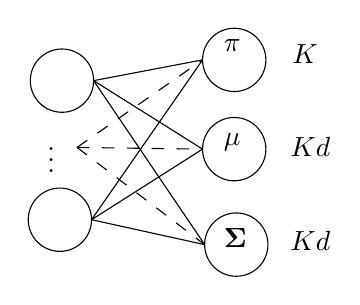
\begin{tikzpicture}[x=0.75pt,y=0.75pt,yscale=-1,xscale=1]
%uncomment if require: \path (0,300); %set diagram left start at 0, and has height of 300

%Shape: Circle [id:dp2684613103597593] 
\draw   (88,112.25) .. controls (88,103.83) and (94.83,97) .. (103.25,97) .. controls (111.67,97) and (118.5,103.83) .. (118.5,112.25) .. controls (118.5,120.67) and (111.67,127.5) .. (103.25,127.5) .. controls (94.83,127.5) and (88,120.67) .. (88,112.25) -- cycle ;
%Shape: Circle [id:dp7515334993320522] 
\draw   (87,179.25) .. controls (87,170.83) and (93.83,164) .. (102.25,164) .. controls (110.67,164) and (117.5,170.83) .. (117.5,179.25) .. controls (117.5,187.67) and (110.67,194.5) .. (102.25,194.5) .. controls (93.83,194.5) and (87,187.67) .. (87,179.25) -- cycle ;
%Shape: Circle [id:dp3956810510931634] 
\draw   (171,102.25) .. controls (171,93.83) and (177.83,87) .. (186.25,87) .. controls (194.67,87) and (201.5,93.83) .. (201.5,102.25) .. controls (201.5,110.67) and (194.67,117.5) .. (186.25,117.5) .. controls (177.83,117.5) and (171,110.67) .. (171,102.25) -- cycle ;
%Shape: Circle [id:dp19016463396194694] 
\draw   (171,145.25) .. controls (171,136.83) and (177.83,130) .. (186.25,130) .. controls (194.67,130) and (201.5,136.83) .. (201.5,145.25) .. controls (201.5,153.67) and (194.67,160.5) .. (186.25,160.5) .. controls (177.83,160.5) and (171,153.67) .. (171,145.25) -- cycle ;
%Shape: Circle [id:dp22276868355052848] 
\draw   (172,191.25) .. controls (172,182.83) and (178.83,176) .. (187.25,176) .. controls (195.67,176) and (202.5,182.83) .. (202.5,191.25) .. controls (202.5,199.67) and (195.67,206.5) .. (187.25,206.5) .. controls (178.83,206.5) and (172,199.67) .. (172,191.25) -- cycle ;
%Straight Lines [id:da20531398432018322] 
\draw    (118.5,112.25) -- (171,102.25) ;
%Straight Lines [id:da5015846339156749] 
\draw    (118.5,112.25) -- (171,145.25) ;
%Straight Lines [id:da38303527040684293] 
\draw    (118.5,112.25) -- (172,191.25) ;
%Straight Lines [id:da4507480129941899] 
\draw    (117.5,179.25) -- (171,102.25) ;
%Straight Lines [id:da05738820526860411] 
\draw    (117.5,179.25) -- (171,145.25) ;
%Straight Lines [id:da686450750606536] 
\draw    (117.5,179.25) -- (172,191.25) ;
%Straight Lines [id:da31471436513544004] 
\draw  [dash pattern={on 4.5pt off 4.5pt}]  (110.5,144.43) -- (171,102.25) ;
%Straight Lines [id:da4379798871611733] 
\draw  [dash pattern={on 4.5pt off 4.5pt}]  (110.5,144.43) -- (171,145.25) ;
%Straight Lines [id:da5452061589510788] 
\draw  [dash pattern={on 4.5pt off 4.5pt}]  (110.5,144.43) -- (172,191.25) ;

% Text Node
\draw (95,135.4) node [anchor=north west][inner sep=0.75pt]    {$\vdots $};
% Text Node
\draw (180,91) node [anchor=north west][inner sep=0.75pt]   [align=left] {$\displaystyle \mathbf{\pi }$};
% Text Node
\draw (180,136.4) node [anchor=north west][inner sep=0.75pt]    {$\mathbf{\mu }$};
% Text Node
\draw (180,182.4) node [anchor=north west][inner sep=0.75pt]    {$\mathbf{\Sigma }$};
% Text Node
\draw (212,138.4) node [anchor=north west][inner sep=0.75pt]    {$Kd$};
% Text Node
\draw (212,183.4) node [anchor=north west][inner sep=0.75pt]    {$Kd$};
% Text Node
\draw (213,93.4) node [anchor=north west][inner sep=0.75pt]    {$K$};


\end{tikzpicture}
\caption{A mixture density output layer. }
\end{figure}

\section{C}

\section{Results?}

\section{The gym environment}

%\clearpage
%\bibliography{ref} 
\end{document}
